\documentclass[10pt,letterpaper]{article}
\usepackage[latin1]{inputenc}
\usepackage{amsmath}
\usepackage{amsfonts}
\usepackage{amssymb}
\usepackage{graphicx}

\renewcommand\thesection{\Alph{section}.}

\title{Z594 Community Ecology\\``Context-dependent'' Interaction Strengths.}

\author{Mark Novak\\mark.novak@oregonstate.edu}
\begin{document}

\maketitle
\section{Empirical motivations \\ Defining species importance.}
\label{EmpMot}
Let's start from an empirical perspective.  How do we define and associate importance to the effects that species have on one another?  Paine (1980) highlighted three ways that ecologists had described networks of species interactions:
\begin{itemize}
\item Connectedness web (topological structure)
\item Energy flow web (material flux)
\item Functional web (effects of species manipulations)
\end{itemize}

\noindent
Paine emphasized how different these perspectives were and how they each led to different conclusions regarding the importance of a species (or interaction) to the community (Fig. \ref{fig:PaineFig}).

\begin{figure}[ht!]
\centering
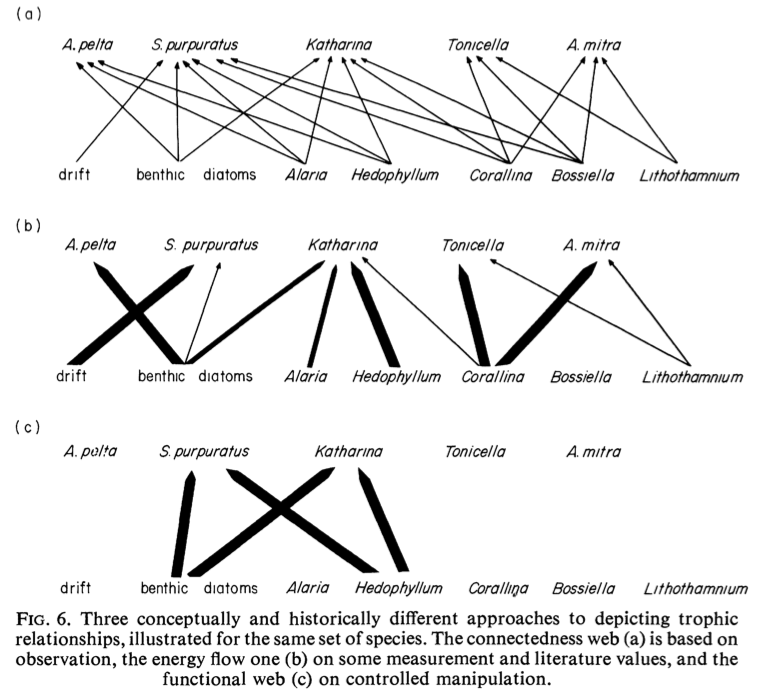
\includegraphics[width=100mm]{figs/Paine1980_Fig6.png}
	\caption{From Paine 1980.}
	\label{fig:PaineFig}

\end{figure}

Among other things, Paine emphasized that \emph{topological structure} could be inferred from observation alone (e.g., watching who eats who).  Many have gone on to use network topology alone in order to ask questions about the importance of species and their interactions by performing hypothetical removal experiments and seeing which additional species subsequently go extinct (i.e. secondary extinctions).  This approach is limited to a bottom-up perspective since removing an apex predator will cause no secondary extinctions.

\emph{Energy (or material) flux webs} were waning in popularity by the time Paine gave his talk.  Mostly this approach was (is) used by ecosystem ecologists in the context of determining energy or nutrient (e.g., carbon or nitrogen) budgets and fluxes between aggregated compartments, but species-resolved networks were also of interest (esp. for higher trophic levels).  This type of study typically used a combination of observational and experimental approaches (but not in the style that Paine popularized).  From this perspective, prey that are abundant typically contribute more (are more important) to the growth of a predator than do rare prey. (More of them are eaten, so there's a greater flux.)  Similarly, abundant predators remove more prey from a prey population than do rare predators, so they tend to be inferred as being more important.

Paine defined \emph{functional webs} as describing the importance of species (or interactions) as evidenced by perturbations to the community.  This approach highlights that it's not just population size but also additional species traits that control a species' importance.  For example, an abundant alga might be nutritionally poor, so although it contributes a lot of carbon to an herbivore (i.e. an important flux) it may contribute little to the herbivore's growth (i.e. a weak effect).  Similarly, a predator might have a voracious appetite and therefore have a large effect on its prey despite being at a very low abundance (e.g., sea otters must consume 20\% of their body weight each day just to survive).  Paine posited that such inferences were not obtainable from observation alone but rather required controlled experimental manipulations.



\section{Per capita effects, Paine's index, and theoretical underpinnings.}
\label{PaineIndex}
A simple manipulative experiment to determine a species' (predator's) importance to its prey might have two treatments:  A $P+$ `control' treatment in which neither prey or predator are manipulated and a $P-$ `manipulated' treatment in which the prey is left as is but the predator population is somehow removed or excluded.  The experiment is run for some amount of time and prey population sizes in each treatment are tracked. The bigger the difference in final population sizes at the end of the experiment, the stronger the interaction between the two species and the more important the predator is considered to be.

Let's associate a model with that experiment.  Suppose that the rate at which the prey population changes over time in the absence of the predator is described by some as yet unspecified function of the prey's own abundance, $g(N)$.  That is,
\begin{equation}
	\lim_{\Delta t \to 0}\frac{\Delta N_{P-}}{\Delta t}=\frac{dN_{P-}}{dt}= g(N)N,
\end{equation}
and that in the presence of the predator it is
\begin{equation}
	\frac{d N_{P+}}{d t} = g(N) N - \alpha N P.
\end{equation}
The function $g(N)$ describes the prey's per capita growth (or mortality) rate.  The product $\alpha N P$ describes the total loss (flux) of prey individuals to the predator population; the higher the population sizes ($N$ and $P$) the higher the loss to the prey population.  Similarly, the higher the per individual (i.e. \emph{per capita}) rate ($\alpha$) with which predator individuals remove  prey individuals, the higher the total loss to the prey population. 

\fbox{
\parbox{100mm}{
\emph{Side note:} Conceivably, if you converted $\alpha N P$ (which has units of numbers of prey per time) to the appropriate energy or material units (e.g., grams of carbon per time), you'd be able to convert between Paine's functional and energy webs.
}}

\subsection{Context dependency or apples and oranges?}
If we were to repeat this experiment in different contexts (e.g., different environmental conditions) we might see a result like the following (Fig. \ref{fig:ExpmtTrtms}):

\begin{figure}[ht!]
\centering
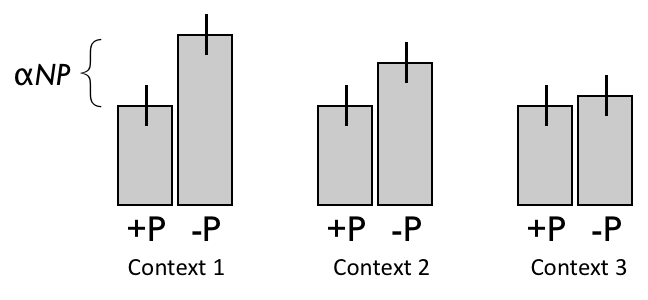
\includegraphics[width=80mm]{figs/Fig1.png}
	\caption{Hypothetical experiments.}
	\label{fig:ExpmtTrtms}
\end{figure}
\noindent
In the literature, such a pattern has frequently been labeled a `context-dependent' species interaction.

However, what if we'd performed this experiment in the field and thus might not have had the same population sizes across the different conditions (i.e. either starting prey abundances or surrounding predator abundances differed).  We might therefore be comparing
\begin{equation*}
\alpha N_1P_1 \;\;vs.\;\; \alpha N_2P_2 \;\; vs. \;\;\alpha N_3P_3, \;\;
\end{equation*}
where in fact either
\begin{equation*}
N_1 \neq N_2 \neq N_3 \;\;\; \text{or} \;\;\; P_1 \neq P_2 \neq P_3.
\end{equation*}
In fact, given our results of Fig. \ref{fig:ExpmtTrtms} it's quite likely that
\begin{equation*}
N_1 < N_2 < N_3 \;\;\; \text{or} \;\;\; P_1 > P_2 > P_3,
\end{equation*}
even if $\alpha$ was the same at all sites.  If that were so, our so-called context dependency would not be surprising at all!

The better question is therefore whether $\alpha$ is constant across conditions. But how can we estimate $\alpha$?  Paine (1992) didn't use a theoretical justification but took the empirically-defensible approach of taking the difference in prey population sizes of the two treatments and dividing by predator and prey population sizes:
\begin{equation}
\text{Paine's index (PI)}=\frac{N_{P+}-N_{P-}}{N_{P-} P} = \frac{\alpha N P}{NP}=\alpha.
\end{equation}
However there is also a `theoretical' way to justify this approach.  Let's assume logistic growth for the prey, $g(N)=r(1-\tfrac{N}{K})$ (i.e. the prey reaches a carrying capacity $K$ in the absence of the predator).  Thus in our two treatments the prey's dynamics are described by
\begin{equation}
	\frac{d N_{P-}}{d t} = rN\left(1-\tfrac{N}{K}\right)
	 \;\;\; \text{and} \;\;\; 	
	 \frac{d N_{P+}}{d t} = rN \left(1-\tfrac{N}{K} - \alpha P \right).
\end{equation}
As time passes the prey populations in the two treatments will eventually reach their respective steady state equilibria:
\begin{equation}
  N_{-P}^*=K  \;\;\; \text{and} \;\;\; N_{+P}^*=K-\alpha PK.
\end{equation}

\fbox{
\parbox{100mm}{
How do we obtain those equilibria?  Let's do it for the $+P$ case:
By definition we know that at equilibrium the population size is no longer changing.  Thus
\begin{equation}
\frac{d N_{P+}}{d t} = rN \left(1-\tfrac{N}{K} - \alpha P \right)=0.
\end{equation}
All we have to do is rearrange this equation to solve for $N$ (which we then refer to as $N^*$ to indicate that we've assumed we're at the equilibrium.)  So, for example,
\begin{eqnarray*} 
rN \left(1-\tfrac{N}{K} - \alpha P \right)=0 \\
rN-\tfrac{rN^2}{K}-r \alpha NP = 0\\
rNK - rN^2 - r \alpha NP K = 0\\
rK - rN -r \alpha P K = 0\\
K-N-\alpha P K=0\\
K-\alpha P K = N\\
N^*= K-\alpha P K.
\end{eqnarray*}
}}
\\[0.2in]
Applying Paine's index using both treatment equilibria gets
\begin{equation}
\text{PI}=\frac{N_{P+}-N_{P-}}{P N_{P-}}=  \frac{K-\alpha P K - K}{PK}=-\alpha.
\end{equation}
Thus we can compare populations from different environmental contexts (or different predator or prey species) that differ in population sizes.  Estimates of $\alpha$ (often referred to as \emph{per capita interaction strengths}, but beware - see Novak et al. 2016) have thus typically been considered `traits' of a species.  For example, \emph{keystone species} may be considered those with the largest $\alpha$, having big effects despite their small population size.  Paine's approach thereby inspired a large amount of empirical effort.

\section{The appearance of context-dependency in per capita effects.}
\label{ApparentContext}
\subsubsection{A slightly different model formulation}
But what if we formulate our model of the predator's effect on prey dynamics in a subtly different way as
\begin{equation}
	\frac{d N_{P-}}{d t} = rN\left(1-\tfrac{N}{K}\right)
\;\;\; \text{and} \;\;\;
\frac{d N_{P+}}{d t} = rN \left(1-\tfrac{N}{K}\right) - \alpha NP.
\end{equation}
The respective equilibria are then
\begin{equation}
  N_{P-}^*=K  \;\;\; \text{and} \;\;\; N_{P+}^*=K-\tfrac{\alpha}{r} PK
\end{equation}
such that Paine's index estimates not $\alpha$ but rather
\begin{equation}
\text{PI}=-\frac{\alpha}{r}.
\end{equation}
Thus, if this is the `correct' description of the interaction and if $r_1 \neq r_2 \neq r_3$ (i.e. the prey's site-specific intrinsic growth rates differ), we would see `context-dependency' across our experiments even if the predator's \emph{per capita attack rate} $\alpha$ (the number of prey eaten per predator per unit time per prey available) were constant. We haven't changed anything about the predator or its `interaction' with the prey, but the predator's effect on the prey now varies across sites.  That would certainly be the case along a productivity gradient, for example. 

It's worth pointing out that $\tfrac{\alpha}{r}$ is a perfectly reasonable per capita measure of an interaction strength:  The effect that a predator has on its prey's population \emph{should} intuitively depend on the \emph{relative} rate at which prey individuals are lost due to predation \emph{versus} the rate at which they are replaced by growth!  (Side-note:  This doesn't mean that our second model is the `better' model!  It simply highlights the importance of considering what model is implicitly being used to describe a focal interaction.  Even empiricists have models in mind, they just might not realize it!)

\subsubsection{A difference in prey life history - Open recruitment}
A second example illustrates the above point too: What if most of the prey population's growth comes from outside immigration or recruitment ($I$).  Let's consider this immigration to be density-independent (i.e. the number of recruits per time doesn't depend on the prey's local abundance).  To simplify things a bit, let's also assume that the prey population's size is sufficiently far from its carrying capacity that it exhibits no self-limitation (i.e. slow exponential growth).  Specifically, when $N<<K$ such that $\left(1-\tfrac{N}{K}\right)\approx 1$, we have
\begin{equation}
	\frac{d N_{P-}}{d t} = I + rN
\;\;\; \text{and} \;\;\;
\frac{d N_{P+}}{d t} = I + rN  - \alpha NP.
\end{equation}
Applying Paine's index gives
\begin{equation}
\text{PI}=\frac{\alpha}{\alpha P-r}.
\end{equation}
Note that this quantity is not a function of the immigration rate as one might have expected. Instead, Paine's index is now dependent on the predator's population size, which is exactly what we were trying to avoid!  Unfortunately, marine systems that are indeed quite open to immigration are the ones to which the index has been applied most frequently! (Table 1 of Novak \& Wootton (2010) shows the consequences of additional model formulations with immigration.)  Think about what that means for how we interpret `context-dependent' patterns!



\section{Nonlinearities and indirect effects.}
What the above two examples indicate is that we have to think about what we mean by a \emph{per capita interaction strength} before we resort to calling something `context-dependent'.  Arguably, each of the above quantities (i.e. $\alpha$, $\tfrac{\alpha}{r}$, $\tfrac{\alpha}{\alpha P-r}$) is a valid per capita measure of an interaction strength!  That is, interaction strengths are not necessarily single values or parameters.  They are better thought of as being functions: functions of abundances, environmental conditions, species traits, and community context (e.g., the presence/absence of other species), etc..

Let's emphasize that with two more examples.


\subsubsection{Nonlinearity}
\label{Nonlinearity}
A predator's functional response $f(N)$ describes how an individual's feeding rate responds to its prey's abundance (Fig.\ref{fig:FuncResp}).
So far we've assumed a linear type I functional response, $f(N)=\alpha N$.  For the saturating type II functional response $\alpha$ only describes the slope at the origin (the per capita attack rate), while the maximum feeding rate is determined by the predator's handling time $h$ (e.g., how long it takes to capture, manipulate, ingest a prey item).  That is,
\begin{equation}
f(N)=\frac{\alpha N}{1+\alpha h N} \;\;\; \text{(type II, $h>0$)}.
\end{equation}
For the type III response in which the prey experiences a `refuge' at low prey densities (e.g., a physical refuge or the predator switches to more abundant prey) the equation is
\begin{equation}
f(N)=\frac{\alpha N^m}{1+\alpha h N^m}. \;\;\; \text{(type III, $h>0, m>1$)}
\end{equation}

\begin{figure}[ht!]
\centering
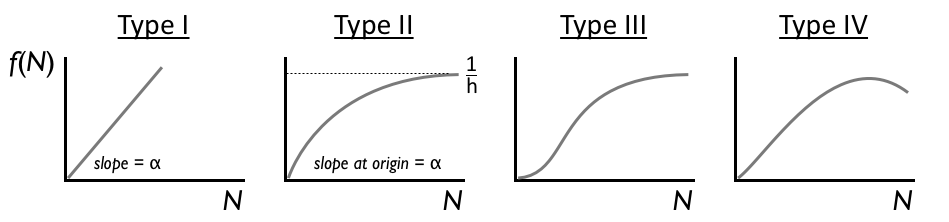
\includegraphics[width=100mm]{figs/FunctionalResponses.png}
	\caption{Holling's type I-III and Ivlev's type IV functional responses.}
	\label{fig:FuncResp}
\end{figure}


For the linear type I response dividing by $N$ gives us $\alpha$, just like we've been talking about thus far.  For the type II, dividing by $N$ shows the per capita effect of the predator on the prey to be $\tfrac{\alpha}{1+\alpha h N}$, which is a declining function of prey abundance (Fig. \ref{fig:PerCapMort}).  For the type III, the per capita effect is first an increasing function and then a decreasing function of $N$ (Fig. \ref{fig:PerCapMort}).

\begin{figure}[ht!]
\centering
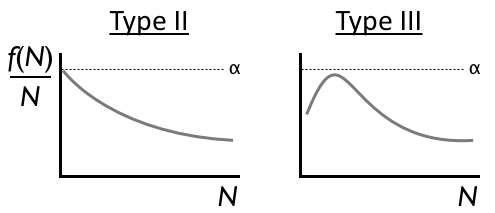
\includegraphics[width=50mm]{figs/PerCapMort.png}
	\caption{Per capita effects.}
	\label{fig:PerCapMort}
\end{figure}


Thus, even in an experiment that holds predator numbers constant, the per capita effect of the predator will change over time as the number of remaining prey individuals declines.  That means that one must not only standardize the treatment $N$'s at the start of an experiment but must also consider how long to run an experiment for.  Different predator species will affect different prey abundances (and thus different apparent per capita effects) depending not only on their $\alpha$'s but also on $h$ and how much they cause the prey population to decline before the experiment is terminated.  The only real solution is to quantify and compare each predator's whole functional response (i.e. both $\alpha$ \emph{and} $h$ parameters), which (typically) requires a different experimental setup than just two treatments (see Novak \& Wootton 2011). 

A frequently suggested alternative (suggested mostly by theoreticians) is to conduct very short `instantaneous' experiments in which $N$ changes very little.  Of course the total predator effect has to be big enough to measure (not to mention statistically `significant'), making this approach largely infeasible.  There's a large literature on estimating the parameters of predator functional responses out there that's relevant to this topic (though note it's largely restricted to artificial lab conditions).

\subsubsection{Indirect effects}
\label{IndirectEffects}
So far we've implicitly considered the focal pair of species to be interacting with each other in isolation of all other species in the community.  There's been no potential for indirect effects mediated by other species (or for \emph{interaction modifications} for that matter).  Let's now consider the interactions of three species.  We'll assume that they each exhibit logistic growth and  interact with each other via exploitative competition (Fig. \ref{fig:3spComp}):
\begin{subequations}
\begin{align}
\frac{1}{N_i}\frac{dN_i}{dt}&=r_-\sum_{j=1}^3 \alpha_{ij}N_j \;\; (i=1,2,3) \\
&=r_i - \alpha_{ii}N_i - \sum_{j\neq i}^2 \alpha_{ij} N_j \;\; (i=1,2,3) \\
&=r_i - \alpha_{ii}N_i - \alpha_{ij} N_j - \alpha_{ik} N_k \;\; (i=1,2,3).
\label{eqn:3spComp}
\end{align}
\end{subequations}
Note three things in these equivalent equations:
\begin{itemize}
\item I've divided both sides by $N$.  Thus the equation represents the per capita growth rate of the $i$th species.
\item  $a_{ii}$ is nothing more than the effect of \emph{intra-specific competition} ($\alpha_{ii}=\tfrac{r_i}{K_i}$) while $\alpha_{ij}$ is the \emph{inter-specific} effect of species $j$ on species $i$.  
\item By changing the $\pm$ signs of some of the $\alpha$'s one could use this scenario represent an intraguild predation (trophic omnivory) scenario as well.
\end{itemize}


In this scenario manipulating the abundance of species $N_1$ will affect the abundance of species $N_2$ not only directly but also indirectly via the response of $N_3$ (Fig. \ref{fig:3spComp}).  To determine what the \emph{net effects} between the species are we start by representing the exact same information about the intra- and interspecific interaction terms of eqn. \ref{eqn:3spComp} in the form of a matrix:
\begin{equation}
A=\left[\begin{array}{ccc}
\alpha_{11} & \alpha_{12} & \alpha_{13} \\
\alpha_{21} & \alpha_{22} & \alpha_{23} \\
\alpha_{31} & \alpha_{32} & \alpha_{33}
\end{array}\right].
\end{equation}

\begin{figure}[ht!]
\centering
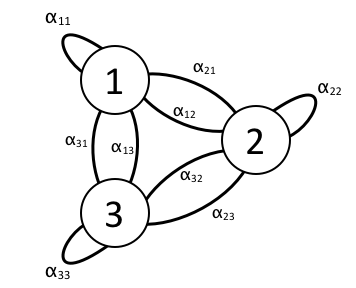
\includegraphics[width=50mm]{figs/3spComp.png}
	\caption{Competitive pairwise interaction strengths between three species.}
	\label{fig:3spComp}
\end{figure}


\noindent
This matrix has seen many names in the literature (see Novak et al. 2016). Let's just call it the \emph{Interaction matrix}.  With some matrix algebra it can be shown that the net effects between species can be calculated by the negative values of the inverse of this matrix ($-A^{-1}$). For our scenario the inverse is

\begin{equation}
-A^{-1}=\left[\begin{array}{ccc}
 \frac{\alpha _{22} \alpha _{33}-\alpha _{23} \alpha _{32}}{det(A)} & \frac{\alpha _{13} \alpha _{32}-\alpha _{12} \alpha _{33}}{det(A)} & \frac{\alpha _{12} \alpha _{23}-\alpha _{13} \alpha _{22}}{det(A)} \\
 \frac{\alpha _{23} \alpha _{31}-\alpha _{21} \alpha _{33}}{det(A)}  & \frac{\alpha _{11} \alpha _{33}-\alpha _{13} \alpha _{31}}{det(A)}  & \frac{\alpha _{13} \alpha _{21}-\alpha _{11} \alpha _{23}}{det(A)}  \\
 \frac{\alpha _{21} \alpha _{32}-\alpha _{22} \alpha _{31}}{det(A)}  & \frac{ \alpha _{12} \alpha _{31}-\alpha _{11} \alpha _{32}}{det(A)}  & \frac{\alpha _{11} \alpha _{22}-\alpha _{12} \alpha _{21}}{det(A)}  \\
\end{array}\right],
\end{equation}
where
\begin{equation*}
det(A)=\alpha _{13} \left(\alpha _{21} \alpha _{32}-\alpha _{22} \alpha _{31}\right)+\alpha _{11} \left(\alpha _{22} \alpha _{33}-\alpha _{23} \alpha _{32}\right)+\alpha _{12} \left(\alpha _{23} \alpha _{31}-\alpha _{21} \alpha _{33}\right).
\end{equation*}
The inverse matrix is read as the net effect on the species in row $i$ that will result from changing the species in column $j$.  (In this case it's implicitly the $j$th species' carrying capacity that is being increased.)  


The net effects matrix looks a bit scary, but note that the matrix determinant, $det(A)$, is common to all elements of the matrix and therefore simply scales the overall magnitude of all species responses.  Therefore it's the numerator of each matrix element that determines whether or not a species in row $i$ will increase or decrease in response a change to the species in column $j$.

Let's focus on just the numerator effect of Species 1 on Species 2 (column 1, row 2):
\begin{equation*}
-A_{21}^{-1} = \frac{\alpha _{23} \alpha _{31}-\alpha _{21} \alpha _{33}}{det(A) }.
\end{equation*}
 We can see that how Sp.2 will respond to a manipulation of Sp.1 depends not only on Sp.1's direct per capita effect ($\alpha_{21}$) but also on how strongly Sp.3 is self-regulated ($\alpha_{33}$) and the strengths of the per capita effects between Sp.3 and the two other species ($\alpha_{23}$ and $\alpha_{31}$).  More specifically, observe that Sp.2 may actually increase in response to an increase in Sp.1 if the indirect effect via Sp.3 ($\alpha_{23} \alpha_{31}$) is greater than the product of their direct interaction ($\alpha_{21}$) and the strength of Sp.3's self-limitation ($\alpha_{33}$).  That should make some intuitive sense: the direct effect \emph{should} logically prevail when Sp.3 is under such strong self-regulation that it doesn't propagate the disturbance.  
 
 To repeat, the effect of Sp.1 on Sp.2 can switch from being negative to positive for reason having nothing to do with their own biology or their own interaction with each other.  Would we really want to say that their interaction itself is therefore `context dependent'?


\section{Food for thought}
So think about what all that means for how we think about, define, or even attempt to quantify the `importance' of a species or the `strength' of its effects and interactions.  And think about what that means for what we might call a `context-dependent' interaction.  On the one hand, everything might be context-dependent when we don't consider the  functional forms and relationships that exist  between parameters (Sec. \ref{PaineIndex} vs. Sec.\ref{ApparentContext}), between parameters and variables (Sec. \ref{Nonlinearity}), or between pairs of species and the rest of their community (Sec. \ref{IndirectEffects}).  An optimistic reductionist (or perhaps a reductionistic optimist?) might argue that context-dependency is only that which is left unexplainable after all these relationships have been accounted for!  

More to the point:  I see as (community) ecology striving to understand of the `rules' that govern the structure and dynamics of systems.  I envision these rules as minimally sufficient descriptions, characterizations, approximations of the various processes that play out in communities; processes like predation, competition, recruitment, etc..  If we are able to sufficiently describe these processes (e.g., characterize their nonlinearities and how their relative rates change as a function of conditions), then we have a predictive ecology. if our predictions fail across some gradient of conditions, then there can only be two reasons:  we don't (yet) understand the rules sufficiently or the rules themselves have changed.  In my view, only the later is \emph{true} `context dependence'.


\end{document}

